% options:
% thesis=B bachelor's thesis
% thesis=M master's thesis
% czech thesis in Czech language
% slovak thesis in Slovak language
% english thesis in English language
% hidelinks remove colour boxes around hyperlinks

\documentclass[thesis=B,english]{FITthesis}[2012/06/26]
\usepackage[utf8]{inputenc} % LaTeX source encoded as UTF-8

\usepackage{cite}
\usepackage{graphicx} %graphics files inclusion
\usepackage{hyperref}
\usepackage{csquotes}
% \usepackage{amsmath} %advanced maths
% \usepackage{amssymb} %additional math symbols

\usepackage{dirtree} %directory tree visualisation
% % list of acronyms
% \usepackage[acronym,nonumberlist,toc,numberedsection=autolabel]{glossaries}
% \iflanguage{czech}{\renewcommand*{\acronymname}{Seznam pou{\v z}it{\' y}ch zkratek}}{}
% \makeglossaries

\newcommand{\tg}{\mathop{\mathrm{tg}}} %cesky tangens
\newcommand{\cotg}{\mathop{\mathrm{cotg}}} %cesky cotangens

\department{Department of Software Engineering}
\title{Open data of Prešov}
\authorGN{Juraj}
\authorFN{Šprlák}
\authorWithDegrees{Juraj Šprlák}
\supervisor{Mgr. Jan Starý, Ph.D.}
\acknowledgements{I would like to thank to my}
\abstractCS{V~několika větách shrňte obsah a přínos této práce v~češtině. Po přečtení abstraktu by se čtenář měl mít čtenář dost informací pro rozhodnutí, zda chce Vaši práci číst.}
\abstractEN{Sem doplňte ekvivalent abstraktu Vaší práce v~angličtině.}
\placeForDeclarationOfAuthenticity{Prague}
\declarationOfAuthenticityOption{4} %volba Prohlášení (číslo 1-6)
\keywordsCS{Otvorené dáta, štátna správa, webová aplikácia, mesto Prešov, Java}
\keywordsEN{Open data, state service, web application, Prešov, Java}

\begin{document}

% \newacronym{CVUT}{{\v C}VUT}{{\v C}esk{\' e} vysok{\' e} u{\v c}en{\' i} technick{\' e} v Praze}
% \newacronym{FIT}{FIT}{Fakulta informa{\v c}n{\' i}ch technologi{\' i}}

\begin{introduction}
	Importance of information is great today. Internet helps us in everyday's life to get the information about almost everything almost immediately. 
	Neither the public affairs did not escape this phenomenon. The society is getting more and more interested in transparency of state government. The idea of Open data was created to satisfy this demand. They can provide the evidence that public money is being well spent and policies are being implemented. Publishing state economy data, public procurements, tax declarations, even fortune of politicians or private companies and other data on public web servers is a common practice in many developed countries.
	\par Thanks mainly to European Union more and more projects targetting electronisation, systematization and publishing the data are being started also in Slovakia. The idea to publish in machine-readable form all that is not secret (or personal data) it still young, though, and often meets unwillingness or incompetence of public institutions. Some of the main flaws of most of the Slovak state and municipalitiy governments published data are their non-machine-readable formats, incompleteness and lack of inteconnectivity.
	Despite these problems, some progress has been made in this area in recent years and the number of datasets published by state institutions grows every day. Thanks to that there is a growing potential for software developers to create applications for manipulating, inteconnecting, analysing and presenting these data and thus turning them into useful information. This is the main goal of this thesis.
	\section*{Open data of Prešov}
	Looking at datasets published on the official website of Slovak government - \href{https://data.gov.sk}{data.gov.sk} one easily disovers, that the most active of all the cities and towns in Slovakia in publishing the data is Prešov. Not only by number of published datasets, but also by quality of the data this city in eastern Slovakia shares the most from its governing with its citizens. These data include all past contracts, invoices, orders and grants of the municipality. That is why these data were chosen for the purpose of this bachelor thesis.
	\section*{Thesis Goals}
	The main goal of this thesis is to analyse, interconnect and present the open data of Prešov municipality to demonstrate their value and usefulness for the citizens. Focus is on interconnecting them by logical ties not only to each other, but also to other published open data in Slovakia, e.g., Slovak Business Register. This requires analyses of all published open data in Slovakia. The final product of the thesis is a web application to present the analysed and interconnected data. The goal is to present the application to Prešov city officials and try to convince them to publish and run it on their web servers, so it can serve the public. The thesis also explains the general concept of open data and all the attributes, that such data need to have.

\end{introduction}

\chapter{Open data}
	This chapter is devoted to the problematics of open data. It provides knowledge about what the open data are, what are their main attributes and explains these attributes.
	\section{Definition}
	\textit{Open data are data that are accessible, can be used, re-used and redistributed by anyone for free (or no more than reproduction cost), subject only, at most, to the requirement to attribute and share-alike.}\cite{opendatahandbook} \linebreak For the sake of interoperability (i.e. ability of diverse systems and organizations to work together) the exact definition of open data is crucial.
	\section{Requirements}
	Requirements that open data need to meet are following:\cite{opendefinition}
	\renewcommand\labelitemii{}
	\begin{itemize}
	 	\item \textbf{Open license}
			\begin{itemize}
				\item The work must be available under an open license. Any additional terms accompanying the work (such as a terms of use, or patents held by the licensor) must not contradict the terms of the license.
		\end{itemize}
  		\item \textbf{Access}
  			\begin{itemize}
  				\item The work shall be available as a whole and at no more than a reasonable one-time reproduction cost, preferably downloadable via the Internet without charge. Any additional information necessary for license compliance (such as names of contributors required for compliance with attribution requirements) must also accompany the work.
  			\end{itemize}
  			\item \textbf{Open Format}
  			\begin{itemize}
  				\item The work must be provided in a convenient and modifiable form such that there are no unnecessary technological obstacles to the performance of the licensed rights. Specifically, data should be machine-readable, available in bulk, and provided in an open format or, at the very least, can be processed with at least one free/libre/open-source software tool.
  			\end{itemize}
	\end{itemize}

To understand the requirements properly, next part is devoted to explaining the most important points mentioned above.
	\subsection{Open licenses}
	Open data need to be available under an open license. A license is open if it:
	\begin{itemize}
		\item allows free use and redistribution (including sale) of the licensed work.
		\item allows creation of derivatives of the work and their distribution under the same terms
		\item does not impose any fee arrangement as part of its conditions
		\item does not discriminate against any person or group
	\end{itemize} 
	\subsection{Data file formats}
	 File format is the digital base in which the information is stored. For the open data to be easily useable, the correct file format is crucial. Choosing the format depends mainly on the character of the data (e.g. structured data for statistics, geodata for geographic data displayed in map, etc.). The formats in which information is published can either be “open” or “closed”. If a file format is “closed”, this may be either because the file format is proprietary and the specification is not publicly available, or because the file format is proprietary and even though the specification has been made public, re-use is limited. If information is released in a closed file format, this can cause significant obstacles to reusing the information encoded in it, forcing those who wish to use the information to buy the necessary software. Open format is a file format with a freely available published specification which places no restrictions, monetary or otherwise, upon its use. The preference from the open government data perspective therefore is that information be released in open file formats which are machine-readable. Following are the data formats that are most-widely used for data publishing by government institutions.\cite{opendatahandbookfileformats}
	 
	 	\subsubsection*{JSON}
	 	JSON is a simple file format that is very easy for any programming language to read. Its simplicity means that it is generally easier for computers to process than others, such as XML.
	 	\subsubsection*{XML}
	 	XML is a widely used format for data exchange because it gives good opportunities to keep the structure in the data and the way files are built on, and allows developers to write parts of the documentation in with the data without interfering with the reading of them.
	 	\subsubsection*{RDF} 	
		RDF makes it possible to represent data in a form that makes it easier to combine data from multiple sources. RDF data can be stored in XML and JSON, among other serializations. RDF encourages the use of URLs as identifiers, which provides a convenient way to directly interconnect existing open data on the Web. RDF is still not widespread, but it has been a trend among Open Government initiatives, including the British and Spanish Government Linked Open Data projects.
		\subsubsection{CSV, XLS/XLSX}
		CSV, or Comma Separated Values can be a very useful format because it is compact and thus suitable to transfer large sets of data with the same structure. It is particularly important for the comma-separated formats that documentation of the individual fields are accurate.
Furthermore it is essential that the structure of the file is respected, as a single omission of a field may disturb the reading of all remaining data in the file without any real opportunity to rectify it, because it cannot be determined how the remaining data should be interpreted.
Many authorities have information left in the spreadsheet, for example Microsoft Excel. In this case, it is stored in XLS format, which is closed (and thus not suitable for open data), or XLSX format, which is partially open. This data can often be used immediately with the correct descriptions of what the different columns mean.
		\subsubsection{Text formats, PDF, TXT}
		Classic documents in formats like Word (closed format), ODF, OOXML, or PDF may be sufficient to show certain kinds of data - for example, relatively stable mailing lists or equivalent. It may be cheap to exhibit in, as often it is the format the data is born in. The format gives no support to keep the structure consistent, which often means that it is difficult to enter data by automated means. Use of templates as the basis of documents is important to make it possible to pull information out of documents.
Plain text documents (.txt) are very easy for computers to read. They generally exclude structural metadata from inside the document however, meaning that developers will need to create a parser that can interpret each document as it appears.
\linebreak \linebreak \linebreak
Most data need further processing (to save the data in the database, connect the data to other sources, etc.). As the data can be too big to manualy process, manipulating with them should be automatable. The best formats for their automatization are the structured ones like JSON, XML and RDF. On the contrary, images and text formats like PDF are very difficult to process. Spreadsheet formats (XLS/XLSX) are structured, but their structure is difficult to follow and data in these formats are usually harder to manipulate.

	\subsection{Data openness levels}
	Tim Berners-Lee, the inventor of the Web and Linked Data initiator, suggested a 5-star deployment scheme for Open Data. This scheme is widely used (e.g., by British government open data) to rate given data based on some of their attributes like file format, structure, inteconnectivity, etc.
\begin{figure}[h!]
  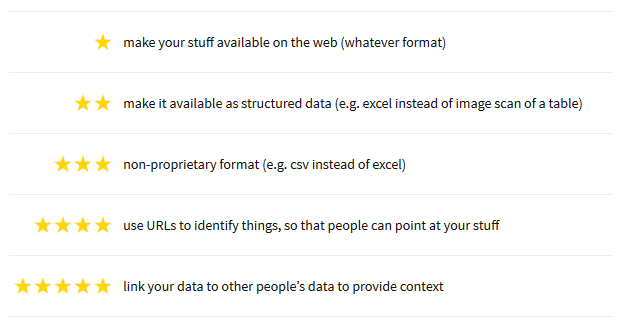
\includegraphics[width=\linewidth]{pictures/5starRating.png}
  \caption{5-star data opennes rating scheme. \cite{5stardata}}
  \label{fig:5-star}
\end{figure}

	\section{Open data success stories}
	Open data barometer is a World Wide Web Foundation's global measure of how governments are publishing and using open data for accountability, innovation and social impact. Barometer ranks governments on:
\begin{itemize}
	\item Readiness for open data initiatives.
	\item Implementation of open data programmes.
	\item Impact that open data is having on business, politics and civil society.\cite{opendatabarometer}
\end{itemize}
The top 5 countries in their last ranking made in 2016 are following:
	\begin{enumerate}
  \item Great Britain
  \item Canada
  \item France
  \item USA
  \item South Korea
  \end{enumerate}
  \subsection{Great Britain's open data}
  Great Britain is the global leader in opening government data. It scored 100 out of 100 in the overal assesment of the prevalence of open data initiatives of Open data barometer.
  There are several reasons why the UK's open data are ranked so well. One of them is its ‘Open Data Readiness’, which is the policy framework for the release of open data. It includes having national guidelines that are applicable to specific sectors, and these guiding principles ensure a smooth release of open data that can benefit anyone that wishes to access it.

Government’s Digital Service Standard provides guidelines on data publishing. A number of regional or city initiatives are integrated into the \href{https://data.gov.uk}{data.gov.uk} portal, too, such as Open Manchester, Leeds Data Mill, Birmingham Open Data, Bristol City Council Open Data, to mention just a few.

The UK Government Licensing Framework (UKGLF) provides a policy and legal framework for licensing the use and re-use of public sector information across the public sector. 

UK’s data portal is unique in the way, it sends automated reminders for datasets. This ensures that data sets are always kept up to date.

Following in the UK’s footsteps in open data guidelines would be a good place to start for other countries hoping to improve in this area.\cite{UKopendatagov}

One of the interesting applications of UK's open data is the \textbf{LMI For All} project. It is an online data portal, developed by the UK Commission for Employment and Skills, which brings together existing national sources of high quality labour market information (LMI) that can inform people’s choices about their careers. The online portal includes LMI that can help answering the questions people ask when thinking about their careers, like how much people earn or what type of persons do what kind of jobs, etc. It includes information from the Annual Survey of Hours and Earnings, the Labour Force Survey, the Employer Skills Survey and Working Futures. All of its data are made freely available  via an Application Programming Interface (API) for use in websites and applications. \linebreak
Other interesting applications built using UK's open data can be seen at \href{https://data.gov.uk/apps}{data.gov.uk/apps}. These include Car Insurance Comparison Application, All GB Railway Stations, Inheritance Tax Calculator UK and more.
\begin{figure}[h!]
\centering
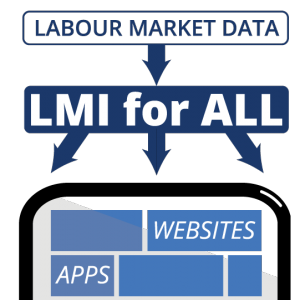
\includegraphics[scale=0.5]{pictures/LMIForAll.png}
  \caption{LMI for all data providing scheme. \cite{lmiforall}}
  \label{fig:LMI for all}
\end{figure}

\subsection{European Union initiatives}
\textbf{Open Data Europe Portal} is the open data portal of the European Union containing datasets that are collected and published by the European Institutions. \linebreak
The \textbf{European Data Portal} is an initiative of the European Commission, and is part of the Digital Single Market. The European Data Portal was created to gather Public Sector Information of the 28 European Member States and the four EFTA countries. Information regarding the provision of data and the benefits of re-using data is also included. Going beyond the harvesting of metadata, the strategic objective of the European Data Portal is to improve accessibility and increase the value of Open Data. Within the Portal, sections are dedicated to: searching datasets, providing data, using data, training and library. It also contains ratings of open data of every involved country. \cite{eudataportal}
	\section{Open data in Slovakia}
	//TODO Political support
	Slovakia ranked 29th in the above mentioned Open data barometer for 2016. It moved 7 places up the ranking since 2015, which indicates, that openning data is on the rise. According to European Data portal factsheet for 2017, a lot of interesting observations were made. Main possitives of Slovak open data initiatives are: presence of action Plan of Open Government for 2017-2019; presence of national guidelines on data publication; data licensing 100\% free of charge and big amount of regional data initiatives. On the contrary, the main negatives/barriers are: less then 25\% of the data are  uploaded automatically; lack of integrated regional portals; passive approach of Open Data holders, mainly by municipalities and lack of promotion of prescribed technical standards. \cite{eudataportalfactsheet}
	\subsection{Slovak open data portal - data.gov.sk}
	Official government open data portal - data.gov.sk was launched in 2013 and according to description present on the website "was created under the Open Government Initiative, which aims to improve governance through increasing transparency, efficiency and accountability". Declared goals of the portal are publishing data and metadata (data describing data like column descriptors, etc.) in machine-readable form using open standards and licenses. Website allows users to search datasets by organizations that publish them, license, file formats and also tags. It also supports full-text search by the name and description of dataset and even by  their location on the map.
	Following are some statistics from the portal (March 2018):
	\begin{itemize}
		\item 4399 unique visitors on average per month
		\item 30\% of the visitors are foreign 
		\item most data sets are available in CSV format
		\item  99\% of the datasets are machine readable
		\item 66 organizations publishing data
		\item 1425 datasets available
	\end{itemize}
	The most active organizations by number of published datasets are following:
\begin{center}
        \begin{tabular}{  p{0.65\linewidth} | c }
        \textbf{Organization} & \textbf{Number of datasets} \\ \hline
        Slovak Statistical Office & 625 \\
        Public Procurement Office & 64 \\
        The city of Prešov & 58 \\
        Ministry of Interior of the Slovak republic & 57 \\
        Central Agricultural Control and Testing Institute & 43 \\
        \end{tabular}
    \end{center}
    \vspace{20px}
    The most commonly used file formats (many datasets are published in more than one file format):
    \begin{center}
        \begin{tabular}{  p{0.65\linewidth} | c }
        \textbf{File format} & \textbf{Number of datasets} \\ \hline
        CSV & 877 \\
        XML & 336 \\
        HTML & 218 \\
        XLSX & 185 \\
        JSON & 11 \\
        \end{tabular}
    \end{center}
    \vspace{20px}
    The most commonly used licenses:
    \begin{center}
        \begin{tabular}{  p{0.65\linewidth} | c }
        \textbf{License} & \textbf{Number of datasets} \\ \hline
        Creative Commons Attribution Share-Alike & 737 \\
        Creative Commons Attribution CCZero & 87 \\
        Creative Commons Attribution Attribution & 24 \\
        Other non-commercial & 14 \\
        GNU Free documentation license & 7 \\
        \end{tabular}
    \end{center}
    \vspace{20px}
    The most common tags:
    \begin{center}
        \begin{tabular}{  p{0.65\linewidth} | c }
        \textbf{Tag} & \textbf{Number of datasets} \\ \hline
        Statistics & 607 \\
        Key tables & 190 \\
        Elections & 177 \\
        Key indicators & 98 \\
        Parliament & 63 \\
        \end{tabular}
    \end{center}
    \subsection{Other state projects}
    Beside above-described official Slovak open data portal, several other big state-run projects are running. The most important ones are Central Register of Contracts and Business register.
    \subsubsection{Central Register of Contracts}
    	Started on 1st January 2011, Central Register of Contracts (available at \href{https://www.crz.gov.sk}{crz.gov.sk}) is a website containing contracts (with their appendices and  attachments) concluded by so-called obliged entities - Government Office, ministries, central government authorities, public bodies and their subordinate organizations (contributors, budgetary organizations, etc.) since the beginning of 2011. As of March 2018, the database contains 1 578 659 contracts. All contracts concluded prior to 2011 are available on older address \href{http://www.zmluvy.gov.sk}{zmluvy.gov.sk}. Operator of the both websites is the Government Office of the Slovak Republic. The register have proven to be successful. The procurement costs of public orders fell by almost one third in the very first year of the register’s operation due to reduced financial mismanagement. Iveta Radičová, former Slovak Prime Minister during whose government the project was started described its success by these words:
\begin{displayquote}“Following the first year of the register’s operation, savings in public finances amounted to an average of 30 percent of costs. There were also some areas – for example, the transport sector – where the savings reached 50 percent. The Office of the Government alone saved EUR 3.5 million in the first year of the register’s operation. The publication of a contract also prevented an overpriced purchase of flowers for EUR 9 million at the Ministry of Education.”
\end{displayquote} \cite{joinupcrz}
    \subsubsection{Business register}   
     The Business Register (available at \href{http://www.orsr.sk}{orsr.sk}) is a public registry that contains particular information specified by the law about individual entrepreneurs, companies and other legal entities. The registry is owned and maintained by the Ministry of Justice of Slovakia. It can be searched by business name, identification number, registered seat, registration number or name of a person. The register provides information from January 2001 onwards.

	\subsection{Non-state initiatives}
	In addition to official projects of Slovak republic and municipalities, there are several civic assosiations, non-profit organizations and private companies dedicated to state open data. Some of them are trying to improve the quality and usefullness of the available data, others are interconnecting them on logical ties with other sources and present them in attractive form. Most often their main goal is to bring more transparency to public spending and state government. Next section looks at the most important ones.
	\subsubsection{Slovensko.digital}
	Slovensko.digital (\href{https://slovensko.digital}{slovensko.digital} is a civic association aimed at improving the quality of state digital services in Slovakia. 
	Their goals are sumarized on their website:
	\begin{displayquote}
		"We want the digital services of the state to be simple, meaningful and have a normal price. We need to increase the transparency and efficiency of spending of public resources as well as the participation of the professional public in the electronisation of public administration."
	\end{displayquote}
	In accordance with these goals, Slovensko.digital set up the \href{https://platforma.slovensko.digital}{platform} for all IT specialists, who want to join the discussions about state IT projects. This civic association's IT specialists systematically rate the state IT projects in one of their project called \href{https://redflags.slovensko.digital/}{Red Flags}. The association is also trying to push for strict rules for new IT projects. They've also started several project as part of \href{https://ekosystem.slovensko.digital/}{ekosystem.slovensko.digital}, some of which provide APIs to public data sources (otherwise only accessible on websites) like Register of legal entities, Central register of contracts, Public procurement journal, Business journal, Registry of financial statements and more.
	\subsubsection{Finstat}
	Finstat was started in 2013 as a web portal, which helps people to freely assess financial health of slovak companies. It connects data from various data sources: ministries, state insurance companies, Business register, Statistical office, Slovak Chamber of executors, Trade Journal, Register of enterpreneurs, Register of financial statements, Register of bankrupts, Czech statistical office and many more and by their processing and analysing provides complex information about slovak companies, individual sectors and groups of enterpreneurs. The portal also helps media and non-profit organizations to analyse companies and investigating corruption cases by development of analyses and making the data of the portal accessible for them. A lot of its features are for free and some features, like APIs access and datasets in CSV are parts of payed packages.
	\subsubsection{Uvostat}
	\href{https://www.uvostat.sk/about}{Uvostat} is a project that processes public procurements data, analyses and presents them in form of statistics and interactive graphs. The statistics include most valuable procurements, most procurements by company or by contracts concluded. The website enables searching in the list of suppliers and even fulltext search in names and contents of the procurements. The interesting fact about the project is that it has been developed by only two people.
	\subsubsection{Otvorené zmluvy (Open contracts)}
	\href{http://www.otvorenezmluvy.sk/o-projekte}{Otvorené zmluvy} is an investigative project of Slovak anti-corruption initiative Aliance Fair-play and Transparency International, which helps citizens to read, search and assess contracts concluded by state and state institutions, which are being published by law since 2011. It offers automated analyses and offers general public to join discussions (crowdsourcing), trying to draw attention to suspicious contracts.	
	\subsubsection{Datanest}
	\href{http://datanest.fair-play.sk/}{Datanest} was also created by Aliance Fair-play as a source of information about management of Slovak public money as part of their anti-corruption initiatives. It serves mainly for journalists, analytics, watchdog organizations, but also for engaged citizens. It contains data generated by state since 1990, which in some cases can't yet be obtained in electronic form elsewhere.
	\subsubsection{foaf.sk}
	\href{http://foaf.sk}{Foaf.sk} draws information about Slovak companies from publicly available Business register, Business journal, Registry of financial statements, database of Social insurance agency debtors, Financial Administration, and other databases. THe website uses graph algorithms to look for and display deeper connections between people and companies in Slovakia, which enables users to quickly search for and display relations between companies and enterpreneurs. The name FOAF comes from the English acronym \textit{Friend Of A Friend} and refers to the phenomenon of the \href{https://en.wikipedia.org/wiki/Small-world_experiment}{small world networks}.
\begin{conclusion}
	%sem napište závěr Vaší práce
\end{conclusion}

\bibliographystyle{csn690}
\begin{thebibliography}{9}
\bibitem{opendatahandbook} 
\textit{What is Open Data? [online].}
[cit. 2018-02-28]. Available from: \url{http://opendatahandbook.org/guide/en/what-is-open-data/} 

\bibitem{opendefinition} 
Open Definition.
\textit{Open Definition 2.0 [online].}
[cit. 2018-03-02]. Available from: \url{http://opendefinition.org/od/2.0/en/} 

\bibitem{europeandataportal} 
European Data Portal.
\textit{What is open data? [online].}
[cit. 2018-03-02]. Available from: \url{https://www.europeandataportal.eu/elearning/en/module1} 

\bibitem{opendatahandbookfileformats}
\textit{File formats [online].}
[cit. 2018-03-02]. Available from: \url{http://opendatahandbook.org/guide/en/appendices/file-formats/} 

\bibitem{5stardata}
\textit{5 star data [online].}
[cit. 2018-23-03]. Available from: \url{http://5stardata.info/en/} 

\bibitem{opendatabarometer}
\textit{Open data barometer [online].}
[cit. 2018-25-03]. Available from: \url{https://opendatabarometer.org/}

\bibitem{UKopendatagov}
\textit{Government Computing [online].}
[cit. 2018-25-03]. Available from: \url{http://central-government.governmentcomputing.com/features/who-is-leading-open-data-in-europe-walking-the-open-data-talk-5653451}

\bibitem{lmiforall}
\textit{LMI for all [online].}
[cit. 2018-25-03]. Available from: \url{http://www.lmiforall.org.uk/about-lmi-for-all/}

\bibitem{eudataportal}
\textit{European Data Portal[online].}
[cit. 2018-25-03]. Available from: \url{https://www.europeandataportal.eu/en/what-we-do/our-activities}

\bibitem{eudataportalfactsheet}
\textit{European Data Portal Factsheet [online].}
[cit. 2018-26-03]. Available from: \url{https://www.europeandataportal.eu/sites/default/files/country-factsheet_slovakia_2017.pdf}

\bibitem{slovakactionplan}
\textit{Action plan of Slovak Open data 2017-2019 [online].}
[cit. 2018-26-03]. Available from: \url{http://www.rokovania.sk/Rokovanie.aspx/BodRokovaniaDetail?idMaterial=26262}

\bibitem{crz}
\textit{Central Registry of Contracts [online].}
[cit. 2018-30-03]. Available from: \url{http://www.vlada.gov.sk/od-1-januara-2011-zacal-fungovat-centralny-register-zmluv/}

\bibitem{joinupcrz}
\textit{Joinup - Slovakian online central register contracts - crs [online].}
[cit. 2018-30-03]. Available from: \url{https://joinup.ec.europa.eu/document/slovakian-online-central-register-contracts-crs}

\bibitem{otvorenezmluvy}
\textit{Otvorené zmluvy [online].}
[cit. 2018-04-04]. Available from: \url{http://www.otvorenezmluvy.sk/o-projekte}

\end{thebibliography}

\chapter{Acronyms}
% \printglossaries
\begin{description}
	\item[GUI] Graphical user interface
	\item[XML] Extensible markup language
	\item[JSON] JavaScript Object Notation
	\item[RDF] Resource Description Framework
	\item[CSV] Comma Separated Values
	\item[PDF] Portable Document Format
	\item[LMI] Labour market information
\end{description}


% % % % % % % % % % % % % % % % % % % % % % % % % % % % 
% % Tuto kapitolu z výsledné práce ODSTRAŇTE.
% % % % % % % % % % % % % % % % % % % % % % % % % % % % 
% 
% \chapter{Návod k~použití této šablony}
% 
% Tento dokument slouží jako základ pro napsání závěrečné práce na Fakultě informačních technologií ČVUT v~Praze.
% 
% \section{Výběr základu}
% 
% Vyberte si šablonu podle druhu práce (bakalářská, diplomová), jazyka (čeština, angličtina) a kódování (ASCII, \mbox{UTF-8}, \mbox{ISO-8859-2} neboli latin2 a nebo \mbox{Windows-1250}). 
% 
% V~české variantě naleznete šablony v~souborech pojmenovaných ve formátu práce\_kódování.tex. Typ může být:
% \begin{description}
% 	\item[BP] bakalářská práce,
% 	\item[DP] diplomová (magisterská) práce.
% \end{description}
% Kódování, ve kterém chcete psát, může být:
% \begin{description}
% 	\item[UTF-8] kódování Unicode,
% 	\item[ISO-8859-2] latin2,
% 	\item[Windows-1250] znaková sada 1250 Windows.
% \end{description}
% V~případě nejistoty ohledně kódování doporučujeme následující postup:
% \begin{enumerate}
% 	\item Otevřete šablony pro kódování UTF-8 v~editoru prostého textu, který chcete pro psaní práce použít -- pokud můžete texty s~diakritikou normálně přečíst, použijte tuto šablonu.
% 	\item V~opačném případě postupujte dále podle toho, jaký operační systém používáte:
% 	\begin{itemize}
% 		\item v~případě Windows použijte šablonu pro kódování \mbox{Windows-1250},
% 		\item jinak zkuste použít šablonu pro kódování \mbox{ISO-8859-2}.
% 	\end{itemize}
% \end{enumerate}
% 
% 
% V~anglické variantě jsou šablony pojmenované podle typu práce, možnosti jsou:
% \begin{description}
% 	\item[bachelors] bakalářská práce,
% 	\item[masters] diplomová (magisterská) práce.
% \end{description}
% 
% \section{Použití šablony}
% 
% Šablona je určena pro zpracování systémem \LaTeXe{}. Text je možné psát v~textovém editoru jako prostý text, lze však také využít specializovaný editor pro \LaTeX{}, např. Kile.
% 
% Pro získání tisknutelného výstupu z~takto vytvořeného souboru použijte příkaz \verb|pdflatex|, kterému předáte cestu k~souboru jako parametr. Vhodný editor pro \LaTeX{} toto udělá za Vás. \verb|pdfcslatex| ani \verb|cslatex| \emph{nebudou} s~těmito šablonami fungovat.
% 
% Více informací o~použití systému \LaTeX{} najdete např. v~\cite{wikilatex}.
% 
% \subsection{Typografie}
% 
% Při psaní dodržujte typografické konvence zvoleného jazyka. České \uv{uvozovky} zapisujte použitím příkazu \verb|\uv|, kterému v~parametru předáte text, jenž má být v~uvozovkách. Anglické otevírací uvozovky se v~\LaTeX{}u zadávají jako dva zpětné apostrofy, uzavírací uvozovky jako dva apostrofy. Často chybně uváděný symbol "{} (palce) nemá s~uvozovkami nic společného.
% 
% Dále je třeba zabránit zalomení řádky mezi některými slovy, v~češtině např. za jednopísmennými předložkami a spojkami (vyjma \uv{a}). To docílíte vložením pružné nezalomitelné mezery -- znakem \texttt{\textasciitilde}. V~tomto případě to není třeba dělat ručně, lze použít program \verb|vlna|.
% 
% Více o~typografii viz \cite{kobltypo}.
% 
% \subsection{Obrázky}
% 
% Pro umožnění vkládání obrázků je vhodné použít balíček \verb|graphicx|, samotné vložení se provede příkazem \verb|\includegraphics|. Takto je možné vkládat obrázky ve formátu PDF, PNG a JPEG jestliže používáte pdf\LaTeX{} nebo ve formátu EPS jestliže používáte \LaTeX{}. Doporučujeme preferovat vektorové obrázky před rastrovými (vyjma fotografií).
% 
% \subsubsection{Získání vhodného formátu}
% 
% Pro získání vektorových formátů PDF nebo EPS z~jiných lze použít některý z~vektorových grafických editorů. Pro převod rastrového obrázku na vektorový lze použít rasterizaci, kterou mnohé editory zvládají (např. Inkscape). Pro konverze lze použít též nástroje pro dávkové zpracování běžně dodávané s~\LaTeX{}em, např. \verb|epstopdf|.
% 
% \subsubsection{Plovoucí prostředí}
% 
% Příkazem \verb|\includegraphics| lze obrázky vkládat přímo, doporučujeme však použít plovoucí prostředí, konkrétně \verb|figure|. Například obrázek \ref{fig:float} byl vložen tímto způsobem. Vůbec přitom nevadí, když je obrázek umístěn jinde, než bylo původně zamýšleno -- je tomu tak hlavně kvůli dodržení typografických konvencí. Namísto vynucování konkrétní pozice obrázku doporučujeme používat odkazování z~textu (dvojice příkazů \verb|\label| a \verb|\ref|).
% 
% \begin{figure}\centering
% 	
\includegraphics[width=0.5\textwidth, angle=30]{cvut-logo-bw}
% 	\caption[Příklad obrázku]{Ukázkový obrázek v~plovoucím prostředí}\label{fig:float}
% \end{figure}
% 
% \subsubsection{Verze obrázků}
% 
% % Gnuplot BW i barevně
% Může se hodit mít více verzí stejného obrázku, např. pro barevný či černobílý tisk a nebo pro prezentaci. S~pomocí některých nástrojů na generování grafiky je to snadné.
% 
% Máte-li například graf vytvořený v programu Gnuplot, můžete jeho černobílou variantu (viz obr. \ref{fig:gnuplot-bw}) vytvořit parametrem \verb|monochrome dashed| příkazu \verb|set term|. Barevnou variantu (viz obr. \ref{fig:gnuplot-col}) vhodnou na prezentace lze vytvořit parametrem \verb|colour solid|.
% 
% \begin{figure}\centering
% 	\includegraphics{gnuplot-bw}
% 	\caption{Černobílá varianta obrázku generovaného programem Gnuplot}\label{fig:gnuplot-bw}
% \end{figure}
% 
% \begin{figure}\centering
% 	\includegraphics{gnuplot-col}
% 	\caption{Barevná varianta obrázku generovaného programem Gnuplot}\label{fig:gnuplot-col}
% \end{figure}
% 
% 
% \subsection{Tabulky}
% 
% Tabulky lze zadávat různě, např. v~prostředí \verb|tabular|, avšak pro jejich vkládání platí to samé, co pro obrázky -- použijte plovoucí prostředí, v~tomto případě \verb|table|. Například tabulka \ref{tab:matematika} byla vložena tímto způsobem.
% 
% \begin{table}\centering
% 	\caption[Příklad tabulky]{Zadávání matematiky}\label{tab:matematika}
% 	\begin{tabular}{|l|l|c|c|}\hline
% 		Typ		& Prostředí		& \LaTeX{}ovská zkratka	& \TeX{}ovská zkratka	\tabularnewline \hline \hline
% 		Text		& \verb|math|		& \verb|\(...\)|	& \verb|$...$|		\tabularnewline \hline
% 		Displayed	& \verb|displaymath|	& \verb|\[...\]|	& \verb|$$...$$|	\tabularnewline \hline
% 	\end{tabular}
% \end{table}
% 
% % % % % % % % % % % % % % % % % % % % % % % % % % % % 

\chapter{Obsah přiloženého CD}

%upravte podle skutecnosti

\begin{figure}
	\dirtree{%
		.1 readme.txt\DTcomment{stručný popis obsahu CD}.
		.1 exe\DTcomment{adresář se spustitelnou formou implementace}.
		.1 src.
		.2 impl\DTcomment{zdrojové kódy implementace}.
		.2 thesis\DTcomment{zdrojová forma práce ve formátu \LaTeX{}}.
		.1 text\DTcomment{text práce}.
		.2 thesis.pdf\DTcomment{text práce ve formátu PDF}.
		.2 thesis.ps\DTcomment{text práce ve formátu PS}.
	}
\end{figure}

\end{document}
